\documentclass[aps,prd,twocolumn,superscriptaddress,nofootinbib,longbibliography,floatfix,showkeys,amsmath,amssymb,10pt]{revtex4-2}

\usepackage{mathptmx}
\usepackage{amsthm}
\usepackage{graphicx}
\usepackage{booktabs}
\usepackage{xcolor}
\usepackage{enumitem}
\usepackage[colorlinks=true,linkcolor=blue!50!black,citecolor=blue!50!black,urlcolor=blue!50!black,bookmarksnumbered=true]{hyperref}
\usepackage{orcidlink}
\usepackage{microtype}
\usepackage{xurl}

\makeatletter
\AtBeginDocument{\def\NAT@bibsetup{\setlength{\labelwidth}{\z@}%
 \setlength{\labelsep}{0.5em}\setlength{\itemindent}{\z@}%
 \setlength{\listparindent}{\z@}\setlength{\topsep}{\z@}%
 \setlength{\parsep}{\z@}\NATx@bibsetup}}
\let\write@bibliographystyle\relax
\let\bibliography@latex\@gobble
\makeatother

\tolerance=2000
\emergencystretch=2em
\hbadness=2000
\hfuzz=1pt
\raggedbottom

\newtheorem{theorem}{Theorem}
\newtheorem{lemma}[theorem]{Lemma}
\newtheorem{proposition}[theorem]{Proposition}
\newtheorem{corollary}[theorem]{Corollary}
\theoremstyle{definition}
\newtheorem{definition}[theorem]{Definition}
\theoremstyle{remark}
\newtheorem{remark}[theorem]{Remark}

\newcommand{\R}{\mathbb{R}}
\newcommand{\Z}{\mathbb{Z}}
\newcommand{\C}{\mathbb{C}}
\newcommand{\cD}{\mathcal{D}}
\newcommand{\HS}{\mathrm{HS}}
\newcommand{\MT}{\mathrm{MT}}
\newcommand{\Gt}{\widetilde G}
\newcommand{\sinc}{\operatorname{sinc}}
\DeclareMathOperator{\tr}{tr}
\DeclareMathOperator{\rank}{rank}
\DeclareMathOperator{\spanop}{span}
\def\zenodoID{10.5281/zenodo.23480714}% DOI of the Zenodo archive (all versions)
\newcommand{\archivelink}{\ifx\zenodoID\empty\url{https://github.com/creelie/mh-phys}%
 \else\href{https://doi.org/\zenodoID}{doi:\zenodoID}\fi}

\setlength{\emergencystretch}{3em}
\begin{document}

\title{More Than 67.32 Percent of the Zeta Zeros Are Simple and on the Critical Line}

\author{Deep Bhattacharjee\,\orcidlink{0000-0003-0466-750X}}
\email{itsdeep@live.com}
\thanks{$*$\,Corresponding author. Second address:
\nolinkurl{d.bhattacharjee@erl-forschung.de}.}
\affiliation{Formerly, Electro-Gravitational Space Propulsion Laboratory
(EGSPL), Bhubaneswar, Odisha 751030, India}
\affiliation{Formerly, University of Calcutta, Senate House, 87/1 College
Street, Kolkata 700073, West Bengal, India}

\author{Ushashi Bhattacharya\,\orcidlink{0009-0002-2254-3914}}
\email{rai.bhattacharya.in@gmail.com}
\affiliation{Formerly, National Taiwan University, Taipei 106319, Taiwan}

\date{19 October 2026}

\begin{abstract}
\itshape
We prove that more than 67.32 percent of the nontrivial zeros of the
Riemann zeta function, counted with multiplicity, are simple and lie on the
critical line, and that the method cannot reach 67.36 percent. The new
ingredient is a sharp bound for the largest eigenvalue of the overlap matrix
of well-separated zeros, which lets long blocks of zeros be used in full.
\par\medskip\upshape\noindent
\textit{2020 Mathematics Subject Classification.} Primary 11M26;
Secondary 11M06, 15A42, 42A05, 65G30.
\end{abstract}

\keywords{Riemann zeta function; simple zeros; pair correlation;
rank--trace inequality}

\maketitle

\makeatletter
\renewcommand\l@subsection[2]{}
\renewcommand\l@subsubsection[2]{}
\makeatother
\tableofcontents

\section{Introduction}\label{sec:intro}

Write $\rho=\beta+i\gamma$ for a nontrivial zero of the Riemann zeta
function, let $N(T_1,T_2)$ be the number of zeros with $T_1<\gamma\le T_2$,
counted with multiplicity, and let $N_0^s(T_1,T_2)$ be the number of those
zeros that are simple and lie on the critical line $\beta=\frac12$. That a
positive proportion of the zeros lie on the line is due to
Selberg~\cite{Sel42}. Levinson's method~\cite{Lev74} gave one third, and the
zeros it detects are simple~\cite{HB79}; Conrey~\cite{Con89} passed two
fifths, Bui, Conrey and Young~\cite{BCY11} passed $41$ percent, and Pratt,
Robles, Zaharescu and Zeindler~\cite{PRZZ20} passed five
twelfths.\footnote{All of these results come from mollified moments of
$\zeta$ or of a combination of its derivatives on the line. The mollifier is
a Dirichlet polynomial chosen to cancel the large values of $\zeta$, and the
proportion grows with its length; the length is limited by the available
estimates for sums of Kloosterman sums. Selberg's original argument already
gave a positive proportion, without an explicit constant; Levinson's constant
is slightly above $0.3474$, and the improvements since then each came from a
longer or more flexible mollifier.}

Montgomery~\cite{Mon73} took a different route. Assuming the Riemann
hypothesis, he evaluated the pair correlation of the zeros against test
functions whose Fourier transform is supported in $[-1,1]$, and deduced that
at least two thirds of the zeros are simple. Montgomery and
Taylor~\cite{Mon75} optimised the test function and reached
\begin{equation}\label{eq:HMT}
 H_\MT:=\frac32-\frac1{\sqrt2}\cot\frac1{\sqrt2}=0.6725007036\ldots,
\end{equation}
which is optimal among certificates of this
shape~\cite{CCLM17}.\footnote{Montgomery's form factor $F(\alpha)$ equals
$|\alpha|+o(1)$ for $|\alpha|\le1$; the zero side of his identity is a sum
over pairs of zeros weighted by a Fourier transform, and on the Riemann
hypothesis every ordinate is real, so a positive test function gives a sum
of positive terms. The window that attains $H_\MT$ is
$\cos(\sqrt2\,t)$ on $[-\frac12,\frac12]$, and the constant is
$2-R(\psi)$, where $R(\psi)$ is the normalised second moment of the window;
see~\cite[Lemma~5.6]{AF26}.}

In 2026 Alp\"oge and Furman~\cite{AF26} removed the Riemann hypothesis from
Montgomery's deduction. They compress Weil's Hermitian form to a family of
modulated copies of a window, split the resulting matrix into a positive
part carried by the zeros on the line and a part of controlled positive index
carried by the off-line pairs, and bound the number of simple zeros on the
line by a rank--trace inequality; the analytic input is the unconditional
pair correlation of Baluyot, Goldston, Suriajaya and
Turnage-Butterbaugh~\cite{BGSTB24}. This gives $\frac23$, and $H_\MT$ with the
Montgomery--Taylor window, unconditionally.\footnote{The paper states that
the argument was found and written by Claude, a language model developed by
Anthropic, and that the authors verified it; it is accompanied by a Lean~4
formalisation. Lamzouri~\cite{Lam26} gave a second proof of the bound
$\frac23$.} A refinement of the rank--trace inequality, which retains a
nonnegative stability defect of the Gram matrix of the simple zeros, and a
certified inequality for seven consecutive zeros, raised the constant to
$0.6730085$~\cite{Ain26}. Our result is the following.

\begin{theorem}\label{thm:main}
As $T\to\infty$,
\begin{align*}
 \liminf_{T\to\infty}\frac{N_0^s(T,2T)}{N(T,2T)}
 &\ge\frac{1000}{993}\Bigl(H_\MT-\frac{19999}{5000000}\Bigr)\\
 &=0.6732133974\ldots .
\end{align*}
\end{theorem}

Summing over dyadic intervals gives the same constant for $N_0^s(0,T)/N(0,T)$.
Figure~\ref{fig:limits} places the bound among the earlier ones.

\begin{figure*}[t]
\centering
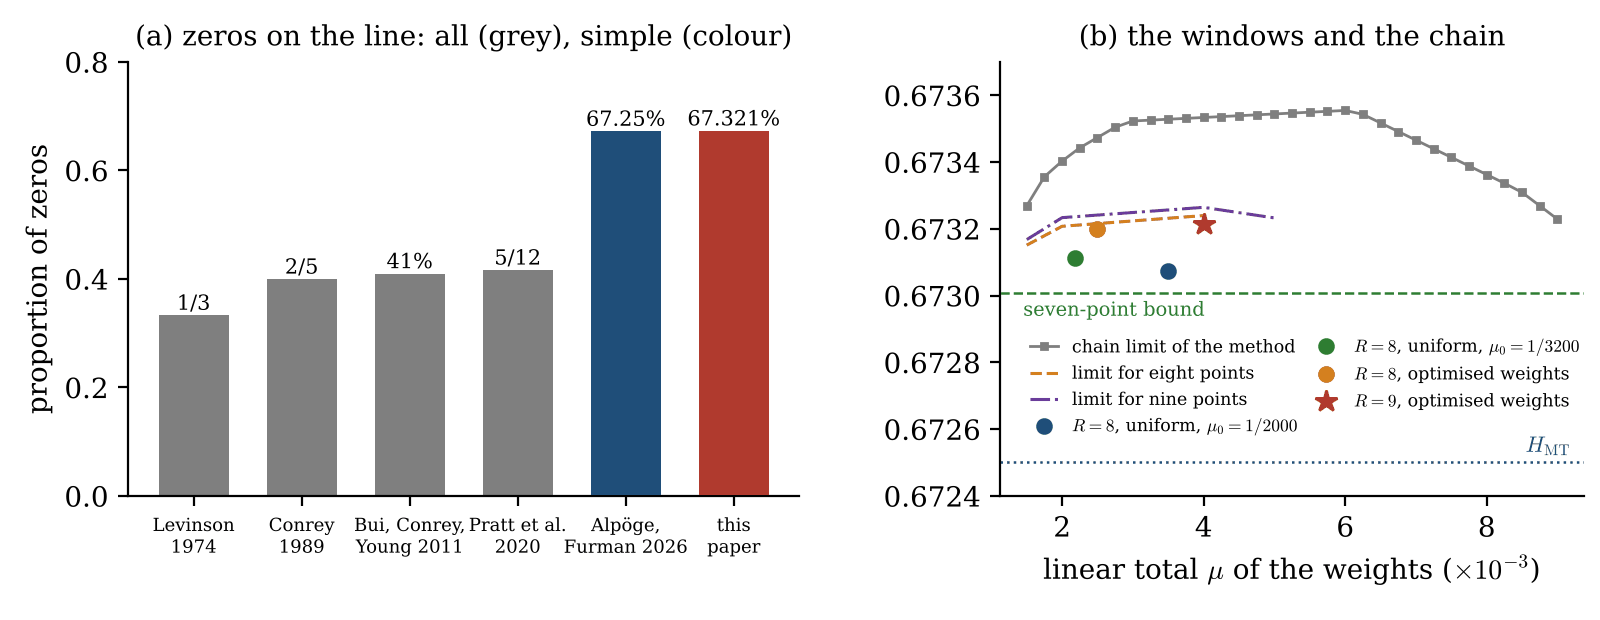
\includegraphics[width=0.96\textwidth]{figures/fig_limits.png}
\caption{(a) Unconditional lower bounds for the proportion of zeros on the
critical line. The grey bars are the proportions of zeros on the line
proved by mollifiers, in the form stated in the titles of the papers; the
coloured bars are proportions of zeros that are both simple and on the line.
(b) The bound $(H_\MT-\mu)/(1-c_0)$ from an inequality for $R$ consecutive
zeros, against the linear total $\mu$ of its weights: the certified points
for $R=8$ with uniform and with optimised weights and for $R=9$ with the
weights of Table~\ref{tab:weights}, the seven-point bound of~\cite{Ain26},
the Montgomery--Taylor constant, the limits for eight and nine points, and
the upper limit of the method obtained from periodic configurations
(Sec.~\ref{sec:limits}).}
\label{fig:limits}
\end{figure*}

The gain over~\cite{Ain26} comes from using the stability defect in full.
For a positive semidefinite matrix $M$ the defect is
$\cD(M)=\tr\Psi(M)$, with $\Psi(t)=(t-1)^2$ on $[0,2]$ and $\Psi(t)=2t-3$
beyond. When every eigenvalue of $M$ is at most $2$, the defect equals
$\tr(M-I)^2$, which for a Gram matrix with unit diagonal is twice the sum of
the squared overlaps of the zeros. Without control of the eigenvalues, the
defect of a block of zeros can only be bounded by $1$, and
in~\cite{Ain26} this cap limits the size of the blocks and hence the gain.
We prove that the overlap matrix of points at mutual distance at least
$\frac{11}{20}$ of the mean spacing has every eigenvalue at most
$1.97903$ (Lemma~\ref{lem:eig}). The bound is sharp: the eigenvalues of
evenly spaced points reach it, and points spaced more closely than
$0.5442$ produce eigenvalues above $2$. Zeros closer than $\frac{11}{20}$
are treated separately: they overlap so strongly that a pair of them alone
has defect at least $0.719$, far more than they cost.

With the cap removed, a block of $m$ zeros has defect proportional to $m$,
and the remaining question is the energy of nine consecutive zeros. Each
pair of the nine zeros enters with a weight that depends on its place in
the window, chosen by linear programming, and with these weights the
inequality sees nearly all the energy that nine consecutive zeros carry.
It is an inequality in eight variables, which we verify by branch and bound in
outward-rounded arithmetic over a table of interval enclosures of the
kernel (Proposition~\ref{prop:window} and Appendix~\ref{app:verify}). The
extremal configurations are close to a lattice with gaps near $1.04$ and
$1.98$, because the overlap kernel vanishes at $1.0573$, $2.0301$ and
$3.0202$.

The method has a limit. Periodic arrangements of zeros satisfy every
constraint the argument uses, and their energy shows that no choice of
window length or weights can push the bound past $0.67357$ (Sec.~\ref{sec:limits}). This
is well below the ceiling $0.6818$ that Alp\"oge and Furman identify for all
certificates based on pair correlation with Fourier support in
$[-1,1]$~\cite[\S7.2]{AF26}.

The route to this argument was found by the learn-from-failure protocol of
Anaxia, the BLLM engine~\cite{Ana26,BB26c}.\footnote{The protocol records
each attempt that fails together with the rule it teaches, and requires
every later attempt to respect the rules so far. Eight rounds preceded this
paper. The direct attacks on the Riemann hypothesis failed and were recorded
as such: a correlation bound below the square-root size of each shift, a
Nyman--Beurling completeness argument that uses only integer dilations, and
shift-by-shift Chowla bounds. Two rules then shaped the present work. The
first was that information beyond pair correlation can be used only where
off-line zeros are provably rare; three-point correlations raise the ceiling
of the method to about $0.709$, but with the zero-density estimates now
known only a gain of $0.0002$ survives, which closed that route. The second
was that a capped block defect saturates near $0.67304$, which pointed to the
uncapped defect and to the eigenvalue bound of Lemma~\ref{lem:eig}. The
engine did not produce the proofs; the failure log, the rules and every
computation are in the archive of this paper (see the data availability
section).} For other approaches to the zeros through spectral and
large-sieve methods, see~\cite{BNFS26,BB26a}.

The paper is organised as follows. Section~\ref{sec:framework} recalls the
framework of~\cite{AF26}. Section~\ref{sec:stability} proves the stability
form of the rank--trace inequality and the pinching inequality.
Section~\ref{sec:kernel} computes the overlap kernel, and
Sec.~\ref{sec:eig} proves the eigenvalue bound. Section~\ref{sec:blocks}
bounds the defect of a block of zeros, Sec.~\ref{sec:window} states the
nine-point inequality, and Sec.~\ref{sec:proof} proves
Theorem~\ref{thm:main}. Section~\ref{sec:limits} shows where the method
stops. Appendix~\ref{app:details} gives the elementary estimates in detail,
and Appendix~\ref{app:verify} describes the verification.

\section{The framework}\label{sec:framework}

We use the notation of Alp\"oge and Furman~\cite{AF26}. Let
\begin{gather*}
 L:=\log\frac T{2\pi},\qquad h:=\frac{2\pi}L,\\
 I:=[T,2T),\qquad I':=[T-\sqrt T,\,2T+\sqrt T),
\end{gather*}
and let $\psi(t)=\cos(\sqrt2\,t)\,\mathbf 1_{[-1/2,1/2]}(t)$ be the
Montgomery--Taylor window. Fix a smooth nondecreasing $\chi$ with $\chi=0$
on $(-\infty,0]$ and $\chi=1$ on $[1,\infty)$, and set
\[
 \phi(u):=\chi\bigl(\tfrac L2+u\bigr)\chi\bigl(\tfrac L2-u\bigr)\,
 \psi(u/L)^{1/2},\qquad
 a:=\frac{\|\phi\|_2^2}L.
\]
With $\widehat f(\xi)=\int f(u)e^{-iu\xi}\,du$, the grid points
$\alpha_k:=T+kh$, and $d:=\lfloor LT/2\pi\rfloor$, each zero $\rho$ gives a
vector
\[
 v_\rho:=\bigl(\widehat\phi(\gamma_\rho-\alpha_k)\bigr)_{0\le k<d},
 \qquad \tilde v_\rho:=\frac{v_\rho}{\sqrt a\,L}.
\]
The matrix $\Gt:=\sum_\rho m_\rho\tilde v_\rho\tilde v_\rho^{\mathsf T}$, the
sum over the zeros with real part of $\gamma_\rho$ in $I'$, is the
compression of Weil's explicit formula to the modulated copies
of $\phi$.\footnote{Weil showed that the Riemann hypothesis is equivalent
to the positivity of the Hermitian form
$W(f,g)=\sum_\rho m_\rho\widehat f(\gamma_\rho)\overline{\widehat
g(\gamma_\rho)}$ on compactly supported test functions~\cite{Wei52}. Off the
line the ordinates $\gamma_\rho$ are complex, and a pair of zeros
$\rho,1-\bar\rho$ contributes an indefinite form of signature $(1,1)$. The
argument of~\cite{AF26} needs no positivity: it counts the positive
directions instead.} Let $s_1$ be the number of simple zeros on the line,
$s_2$ the number of distinct multiple zeros on the line, and $p$ the number
of pairs $\{\rho,1-\bar\rho\}$ off the line, all with real part of the
ordinate in $I'$. Let $V$ be the $d\times s_1$ matrix whose columns are the
vectors $\tilde v_\rho$ of the simple zeros on the line, and put
\[
 P_1:=VV^{\mathsf T},\qquad Q':=\Gt-P_1,\qquad M:=V^{\mathsf T}V.
\]

\begin{proposition}[\cite{AF26}]\label{prop:AF}
As $T\to\infty$:
\begin{enumerate}[label=(\alph*),leftmargin=*]
\item every column of $V$ has norm at most $1$, $n_+(Q')\le s_2+p$, and
 $s_1+2s_2+2p\le N(I')$;
\item $\tr\Gt=N(T,2T)+o(N(T,2T))$;
\item $\|\Gt\|_\HS^2=(2-H_\MT+o(1))\,N(T,2T)$;
\item for all $z,z'\in\C$,
 $\sum_{k\in\Z}\widehat\phi(z-\alpha_k)\widehat\phi(z'-\alpha_k)=
 L\,\widehat{\phi^2}(z-z')$, and
 $|\widehat\phi(r)|\ll\min(L,r^{-2})$ for real $r$.
\end{enumerate}
\end{proposition}

\begin{proof}
Part (a) is Lemma~2.1 at $z=z'=\gamma_\rho$, Proposition~4.1 and the
decomposition in the proof of Theorem~A in~\cite{AF26}. Part (b) is
Proposition~4.2 there together with $N(I')-N(I)\ll\sqrt T\log T$. Part (c)
is Theorem~5.7 with Lemma~5.6, since $R(\psi)=2-H_\MT$ for the
Montgomery--Taylor window. Part (d) is Lemma~2.1 and the bound~(2.8)
of~\cite{AF26}.
\end{proof}

Here $n_+$ is the number of positive eigenvalues and $\|X\|_\HS^2=\tr X^2$.
Proposition~\ref{prop:AF}(b) and (c) are where the prime numbers enter:
(c) is Montgomery's second moment, evaluated without the Riemann
hypothesis~\cite{BGSTB24}.

\section{The stability defect}\label{sec:stability}

Define the convex function
\[
 \Psi(t):=\begin{cases}(t-1)^2,&0\le t\le2,\\ 2t-3,&t\ge2,\end{cases}
\]
and, for a positive semidefinite matrix $X$, the stability defect
$\cD(X):=\tr\Psi(X)\ge0$. The function $\Psi$ is continuously
differentiable, with $\Psi'(2)=2$ from both sides.

\begin{lemma}[Rank--trace inequality with defect]\label{lem:stable}
Let $V$ be a $d\times r$ matrix whose columns have norm at most $1$, put
$P=VV^*$ and $M=V^*V$, and let $Q$ be Hermitian with $n_+(Q)\le b$. Then
\[
 \|P+Q\|_\HS^2\ge4\tr(P+Q)-3r-4b+\cD(M).
\]
\end{lemma}

The case $\cD(M)=0$ is the rank--trace inequality of~\cite[Lemma 3.2]{AF26};
the defect term is the refinement of~\cite{Ain26}. We give the proof.

\begin{proof}
Write $Q=Q_+-Q_-$ with $Q_\pm\succeq0$, $Q_+Q_-=0$ and $\rank Q_+\le b$.
Since $\tr(PQ_+)\ge0$ and $\tr(Q_+Q_-)=0$,
\[
 \|P+Q\|_\HS^2\ge\|P-Q_-\|_\HS^2+\|Q_+\|_\HS^2.
\]
Every positive eigenvalue $q$ of $Q_+$ satisfies $q^2\ge4q-4$, so
$\|Q_+\|_\HS^2\ge4\tr Q_+-4b$. Let $p_1\ge\dots\ge p_d\ge0$ be the
eigenvalues of $P$; the first $r$ of them are the eigenvalues of $M$ and the
others vanish. Let $n_1\ge\dots\ge n_d\ge0$ be the eigenvalues of $Q_-$.
Von Neumann's trace inequality $\tr(PQ_-)\le\sum_ip_in_i$ gives
\[
 \|P-Q_-\|_\HS^2+4\tr Q_-\ge\sum_{i\le r}\bigl((p_i-n_i)^2+4n_i\bigr),
\]
because the terms with $i>r$ are $n_i^2+4n_i\ge0$. For $p\ge0$,
\[
 \min_{n\ge0}\bigl((p-n)^2+4n\bigr)=2p-1+\Psi(p),
\]
the minimum being at $n=0$ when $p\le2$ and at $n=p-2$ when
$p\ge2$.\footnote{For $p\le2$ the minimum is $p^2=2p-1+(p-1)^2$, and for
$p\ge2$ it is $4+4(p-2)=4p-4=2p-1+(2p-3)$. The function $\Psi$ is thus the
exact loss in the scalar inequality $p^2\ge2p-1$ when one allows a
compensating negative eigenvalue; this is what makes the defect the right
quantity to keep.} Hence
$\|P-Q_-\|_\HS^2\ge2\tr P-r+\cD(M)-4\tr Q_-$. Adding the two bounds,
\[
 \|P+Q\|_\HS^2\ge4\tr(P+Q)-2\tr P-r-4b+\cD(M),
\]
and $\tr P=\sum\|v_j\|^2\le r$.
\end{proof}

\begin{lemma}[Pinching]\label{lem:pinch}
Let $X\succeq0$ be an $n\times n$ matrix and let $B_1,\dots,B_q$ be a
partition of $\{1,\dots,n\}$. Then
$\cD(X)\ge\sum_{j}\cD(X_{B_jB_j})$, where $X_{BB}$ is the principal
submatrix on $B$.
\end{lemma}

\begin{proof}
Let $\Pi_j$ be the coordinate projection onto $B_j$ and, for
$\varepsilon\in\{\pm1\}^q$, let $U_\varepsilon=\sum_j\varepsilon_j\Pi_j$.
Then $\sum_j\Pi_jX\Pi_j=2^{-q}\sum_\varepsilon U_\varepsilon XU_\varepsilon$.
The map $Y\mapsto\tr\Psi(Y)$ is convex on positive semidefinite matrices,
since $\Psi$ is convex on $[0,\infty)$~\cite[Theorem V.2.5]{Bha97}, and it
is unitarily invariant. Hence
$\cD(\sum_j\Pi_jX\Pi_j)\le\cD(X)$, and the left side is
$\sum_j\cD(X_{B_jB_j})$.
\end{proof}

\begin{corollary}\label{cor:defect}
Let $M^\circ$ be the principal submatrix of $M$ indexed by any set of simple
zeros on the line with ordinates in $I'$. Then
\[
 N_0^s(T,2T)\ge H_\MT\,N(T,2T)+\cD(M^\circ)-o(N(T,2T)).
\]
\end{corollary}

\begin{proof}
Apply Lemma~\ref{lem:stable} to $P_1+Q'=\Gt$ with $r=s_1$ and
$b=s_2+p$ (Proposition~\ref{prop:AF}(a)):
\begin{align*}
 \|\Gt\|_\HS^2&\ge4\tr\Gt-3s_1-4s_2-4p+\cD(M)\\
 &\ge4\tr\Gt-s_1-2N(I')+\cD(M).
\end{align*}
By Proposition~\ref{prop:AF}(b), (c) and $N(I')=N(T,2T)+o(N(T,2T))$, this is
$s_1\ge H_\MT N(T,2T)+\cD(M)-o(N(T,2T))$. Lemma~\ref{lem:pinch}, applied
to $M^\circ$ and its complement, gives $\cD(M)\ge\cD(M^\circ)$, and
$N_0^s(T,2T)\ge s_1-O(\sqrt T\log T)$.
\end{proof}

\section{The overlap kernel}\label{sec:kernel}

Put
\begin{gather*}
 K(x):=\int_{-1/2}^{1/2}\cos(\sqrt2\,t)\cos(2\pi xt)\,dt,\\
 k(x):=\frac{K(x)}{K(0)},\qquad w:=k^2,
\end{gather*}
so that $K(0)=K_0:=\sqrt2\sin(1/\sqrt2)=0.9187253698\ldots$ and
\begin{equation}\label{eq:Kexplicit}
 K(x)=\frac12\Bigl(\sinc\bigl(\pi x-\tfrac1{\sqrt2}\bigr)
 +\sinc\bigl(\pi x+\tfrac1{\sqrt2}\bigr)\Bigr),
\end{equation}
with $\sinc s=(\sin s)/s$. For a simple zero $\rho$ on the line put
$x_\rho:=(\gamma_\rho-T)/h$, its ordinate measured in units of $h$, which
is the mean spacing of the zeros up to a factor $1+O(1/L)$.

\begin{lemma}\label{lem:kernel}
Retain the simple zeros on the line with $x_\rho\in[L^2,d-L^2]$. The
others number $o(N(T,2T))$ among those in $I$, and for every fixed $S>0$,
uniformly for retained zeros with $|x_\rho-x_{\rho'}|\le S$,
\[
 \langle\tilde v_\rho,\tilde v_{\rho'}\rangle=k(x_\rho-x_{\rho'})+o(1).
\]
\end{lemma}

\begin{proof}
By Proposition~\ref{prop:AF}(d), the sum over all $k\in\Z$ equals
$(aL)^{-1}\widehat{\phi^2}(hx)$ with $x=x_\rho-x_{\rho'}$. The grid points
outside $[0,d)$ lie at distance at least $hL^2=2\pi L$ from $\gamma_\rho$
and $\gamma_{\rho'}$, so by Cauchy--Schwarz and the decay of
$\widehat\phi$ they contribute
$\ll L^{-2}\sum_{j\ge0}(2\pi L+jh)^{-4}\ll L^{-4}$ after division by
$aL^2$. For the full sum, the substitution $u=Lt$ gives
\[
 \frac{\widehat{\phi^2}(hx)}{aL}=
 \frac{\int\phi(Lt)^2e^{-2\pi ixt}\,dt}{\int\phi(Lt)^2\,dt}.
\]
As $T\to\infty$, $\phi(Lt)^2\to\psi(t)$ in $L^1$, because the two factors
$\chi$ differ from $1$ only on a set of $t$ of measure $O(1/L)$. The ratio
therefore tends to $K(x)/K_0$, uniformly for $|x|\le S$. The deleted zeros
have ordinates in two intervals of length $2\pi L$ at the ends of $I$, and
there are $O(L^2)$ of them by $N(t,t+1)\ll\log t$~\cite[Theorem
9.2]{Tit86}.
\end{proof}

The kernel has three properties that the argument uses (Fig.~\ref{fig:kernel}).

\begin{lemma}\label{lem:kprops}
\begin{enumerate}[label=(\roman*),leftmargin=*]
\item $k(0)=1$, $|k|\le1$, and $k$ is decreasing on $[0,1]$.
\item $w(x)\ge w(\frac{11}{20})=0.3595640596\ldots$ for $0\le x\le\frac{11}{20}$.
\item The first three positive zeros of $k$ are $1.0572782\ldots$,
 $2.0300675\ldots$ and $3.0202429\ldots$, and $w(x)=O(x^{-2})$.
\end{enumerate}
\end{lemma}

\begin{proof}
(i) $|K(x)|\le\int\cos(\sqrt2t)\,dt=K_0$. For $0<x\le1$ and
$0<t\le\frac12$ one has $0<2\pi xt\le\pi$, so
\[
 K'(x)=-\int_{-1/2}^{1/2}2\pi t\cos(\sqrt2t)\sin(2\pi xt)\,dt<0.
\]
(ii) follows from (i) and $k(\frac{11}{20})>0$; the value is computed in
Appendix~\ref{app:details}. (iii) The zeros are those of~\eqref{eq:Kexplicit};
the decay follows from the same formula.
\end{proof}

\begin{figure*}[t]
\centering
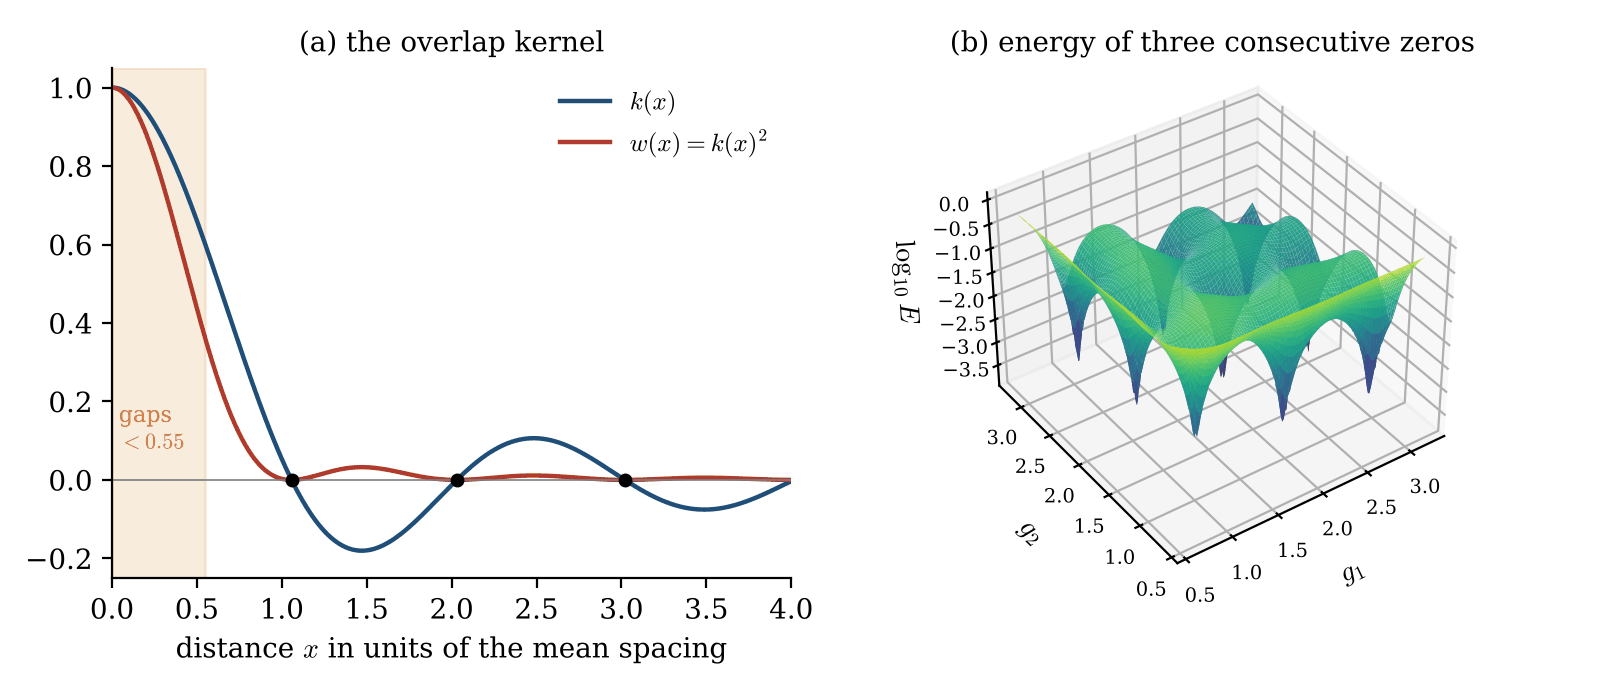
\includegraphics[width=0.96\textwidth]{figures/fig_kernel.png}
\caption{(a) The overlap kernel $k$ and its square $w$, in units of the mean
spacing; the dots are the zeros of $k$, near $1$, $2$ and $3$. The shaded
strip marks the gaps below $\frac{11}{20}$, where the eigenvalue bound of
Lemma~\ref{lem:eig} no longer applies and zeros are treated as clusters.
(b) The energy $E=2[w(g_1)+w(g_2)+w(g_1+g_2)]$ of three consecutive zeros
with gaps $g_1,g_2$, on a logarithmic scale. Its valleys follow the zeros of
$k$; the extremal configurations of Proposition~\ref{prop:window} sit in
these valleys, with gaps near $1.04$ and $1.98$.}
\label{fig:kernel}
\end{figure*}

\section{Separated zeros}\label{sec:eig}

\begin{lemma}\label{lem:eig}
Let $\delta_1=\frac{11}{20}$ and let $x_1,\dots,x_n$ be real numbers with
$|x_i-x_j|\ge\delta_1$ for $i\ne j$. Then every eigenvalue of the matrix
$\bigl(k(x_i-x_j)\bigr)_{i,j}$ lies in
\[
 \Bigl[0,\ \frac1{\delta_1K_0}\Bigr]=[0,\,1.9790264\ldots].
\]
\end{lemma}

\begin{proof}
For a real vector $c$, with $S(t)=\sum_jc_je^{2\pi ix_jt}$,
\[
 \sum_{i,j}c_ic_jk(x_i-x_j)=\frac1{K_0}\int_{-1/2}^{1/2}\cos(\sqrt2\,t)
 \,|S(t)|^2\,dt\ge0,
\]
because the cosine is positive on $[-\frac12,\frac12]$. Let
$\Lambda(t)=\sinc^2(\pi\delta_1t)$. Its Fourier transform is the triangle
\[
 \int_\R\Lambda(t)e^{2\pi i\xi t}\,dt=\frac1{\delta_1}
 \Bigl(1-\frac{|\xi|}{\delta_1}\Bigr)_+,
\]
which vanishes for $|\xi|\ge\delta_1$. We show in Appendix~\ref{app:details}
that
\begin{equation}\label{eq:majorant}
 \Lambda(t)\ge\cos(\sqrt2\,t)\qquad\text{for }|t|\le\tfrac12 .
\end{equation}
Since $\Lambda\ge0$ everywhere, $\Lambda$ majorises
$\cos(\sqrt2\,t)\mathbf 1_{[-1/2,1/2]}$ on the whole line, so
\begin{align*}
 \int_{-1/2}^{1/2}\cos(\sqrt2t)|S|^2\,dt&\le\int_\R\Lambda|S|^2\,dt\\
 &=\sum_{i,j}c_ic_j\widehat\Lambda(x_i-x_j)=\frac{\|c\|^2}{\delta_1},
\end{align*}
because $\widehat\Lambda(x_i-x_j)=0$ for $i\ne j$.\footnote{This is the
mechanism of the large sieve: a band-limited majorant of the weight turns a
quadratic form over separated points into its diagonal. Beurling and Selberg
chose the majorant to optimise the large sieve constant;
see~\cite{Vaa85}. Here the weight is $\cos(\sqrt2t)$ on an interval of
length $1$ rather than the indicator, and the separation $\delta_1$ is below
$1$, the range in which the classical constant $1+1/\delta$ exceeds $2$ and
is useless for us. The Fej\'er kernel $\Lambda$ with exactly the bandwidth
$\delta_1$ wins because $\cos(\sqrt2t)$ is flat to second order at $t=0$,
where $\Lambda$ has curvature $-(\pi\delta_1)^2/3\approx-0.995$, almost the
$-1$ of the cosine.} Dividing by $K_0$ gives the upper bound.
\end{proof}

The constant is sharp. For the points $x_j=j\delta$, $1\le j\le n$, and the
vector of ones, the Rayleigh quotient is
$\sum_{|\ell|<n}(1-|\ell|/n)\,k(\ell\delta)$, the $n$-th Fej\'er mean at
$0$ of the Fourier series of the $1$-periodic function
$\theta\mapsto(\delta K_0)^{-1}\sum_{j\in\Z}\psi((j-\theta)/\delta)$ by
Poisson summation. For $\delta<2$ only the term $j=0$ is nonzero near
$\theta=0$, the function is continuous there with value $1/(\delta K_0)$, and
Fej\'er's theorem gives $\lambda_{\max}\ge1/(\delta K_0)-o(1)$ as
$n\to\infty$. So lattices with spacing below the critical value
\[
 \delta^*=\frac1{2K_0}=0.5442322\ldots
\]
have eigenvalues above $2$, and Lemma~\ref{lem:eig} cannot hold with
$\frac12$ in place of $\frac{11}{20}$. Figure~\ref{fig:majorant} shows the
majorant and the eigenvalues of lattices.

\begin{figure*}[t]
\centering
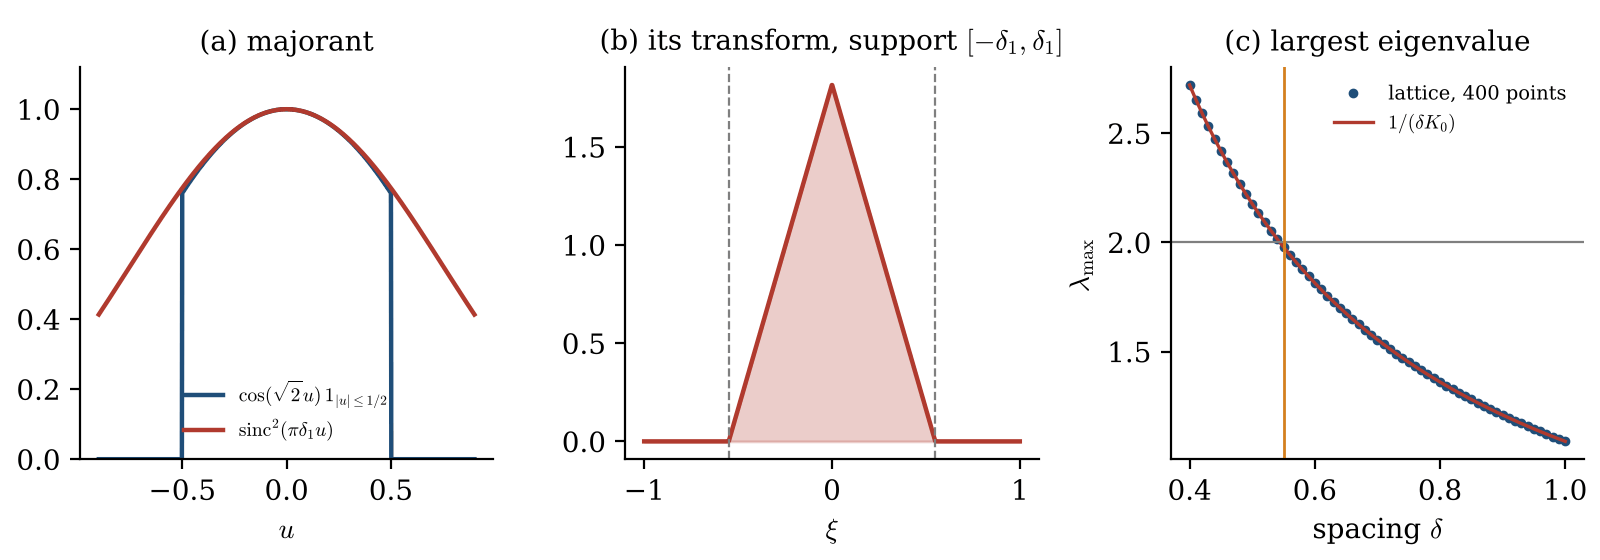
\includegraphics[width=0.96\textwidth]{figures/fig_majorant.png}
\caption{The eigenvalue bound. (a) The Fej\'er kernel
$\sinc^2(\pi\delta_1u)$ lies above the Montgomery--Taylor window on
$[-\frac12,\frac12]$; the two curves agree to second order at $u=0$.
(b) Its Fourier transform, a triangle supported in $[-\delta_1,\delta_1]$,
so that points at distance at least $\delta_1$ do not interact.
(c) The largest eigenvalue of the overlap matrix of $400$ evenly spaced
points against the spacing $\delta$, with the bound $1/(\delta K_0)$; the
vertical line is $\delta_1=\frac{11}{20}$ and the horizontal line is the
threshold $2$ of the defect.}
\label{fig:majorant}
\end{figure*}

\section{The defect of a block of zeros}\label{sec:blocks}

Fix an integer $R\ge2$. A system of weights for $R$ points consists of
numbers $b_1,\dots,b_{R-1}>0$ and $a_{r,i}\ge0$, for $1\le r\le R-1$ and
$0\le i\le R-1-r$, such that
\begin{equation}\label{eq:weights}
 \sum_{i=1}^{R-1}b_i=\mu,\qquad
 \sum_{i=0}^{R-1-r}a_{r,i}\le2\quad(1\le r\le R-1);
\end{equation}
we call $\mu$ the linear total of the weights. For gaps
$g=(g_1,\dots,g_{R-1})$ in $[0,\infty)^{R-1}$ put $y_0=0$,
$y_i=g_1+\dots+g_i$, and
\begin{equation}\label{eq:FR}
 F(g):=\sum_{i=1}^{R-1}b_ig_i+\sum_{r=1}^{R-1}
 \sum_{i=0}^{R-1-r}a_{r,i}\,w(y_{i+r}-y_i).
\end{equation}
The second sum runs over all pairs of the $R$ points $y_0<\dots<y_{R-1}$,
and the pair $(y_i,y_{i+r})$ carries the weight $a_{r,i}$, which depends on
its place in the window. The uniform weights $b_i=\mu_0$,
$a_{r,i}=2/(R-r)$ give the function $F_R$ used in~\cite{Ain26}, with
$\mu=(R-1)\mu_0$.\footnote{Every system of weights gives the same totals in
the proof of Lemma~\ref{lem:windows}; what the weights change is the
minimum of a single window. The extremal configurations of $F_R$ do not
use all places alike: some pairs sit near a zero of $k$ at every
near-minimal configuration and contribute almost nothing, while others
always carry a visible overlap. Moving weight from the first kind of place
to the second raises the minimum.}

\begin{lemma}\label{lem:windows}
Suppose that $F\ge c_0$ on $[0,\infty)^{R-1}$ for a system of weights with
linear total $\mu$. Then for all real $y_1<\dots<y_n$,
\[
 2\sum_{i<j}w(y_j-y_i)+\mu\,(y_n-y_1)\ge c_0\,(n-R+1).
\]
\end{lemma}

\begin{proof}
For $n<R$ the right side is not positive. For $n\ge R$, add the inequality
$F\ge c_0$ over the $n-R+1$ windows $y_s,\dots,y_{s+R-1}$ of $R$
consecutive points. A pair $y_j,y_{j+r}$ with $r<R$ sits at the place
$i=j-s$ of the window that starts at $s$, and different windows give
different places, so its total weight is at most $\sum_ia_{r,i}\le2$;
pairs at least $R$ steps apart do not occur and $w\ge0$. In the same way
the gap $y_{j+1}-y_j$ is the $i$-th gap of at most one window for each $i$,
so the linear terms add up to at most $\mu(y_n-y_1)$.
\end{proof}

For a set $B$ of retained simple zeros, let $G_B$ be its Gram matrix
$(\langle\tilde v_\rho,\tilde v_{\rho'}\rangle)_{\rho,\rho'\in B}$ and let
$\spanop(B)$ be the difference between the largest and the smallest
$x_\rho$ in $B$.

\begin{proposition}\label{prop:block}
Suppose that $F\ge c_0$ on $[0,\infty)^{R-1}$ for a system of weights with
linear total $\mu$, and that
\begin{equation}\label{eq:c0cond}
 (R+1)\,c_0\le\tfrac43\,w(\tfrac{11}{20}).
\end{equation}
Fix $m\ge R$. Then, uniformly over all sets $B$ of
$m$ consecutive retained simple zeros on the line,
\[
 \cD(G_B)+\mu\spanop(B)\ge c_0\,(m-R+1)-o(1).
\]
\end{proposition}

\begin{proof}
If $\mu\spanop(B)\ge c_0(m-R+1)$ there is nothing to prove, since
$\cD\ge0$. Otherwise $\spanop(B)<S:=c_0(m-R+1)/\mu$, so by
Lemma~\ref{lem:kernel} every entry of $G_B$ is
$k(x_\rho-x_{\rho'})+o(1)$, uniformly in $B$. Write
$y_1<\dots<y_m$ for the points $x_\rho$, $\rho\in B$.

Call a gap $y_{i+1}-y_i$ short if it is less than $\delta_1=\frac{11}{20}$.
A cluster is a maximal set of at least two consecutive points joined by
short gaps; let there be $q$ clusters, of sizes $s_1,\dots,s_q\ge2$. The
points outside the clusters fall into at most $q+1$ maximal sets of
consecutive points, the runs, of sizes $n_1,n_2,\dots$; inside a run every
gap is at least $\delta_1$, so all distances are. Split each cluster into
$\lfloor s_j/2\rfloor$ pairs of consecutive points and, when $s_j$ is odd,
one single point. Runs, pairs and single points partition $B$
(Fig.~\ref{fig:blocks}), and Lemma~\ref{lem:pinch} gives
\[
 \cD(G_B)\ge\sum_{\text{runs}}\cD(G_{\text{run}})
 +\sum_{\text{pairs}}\cD(G_{\text{pair}}).
\]
The function $X\mapsto\cD(X)$ is uniformly continuous on the matrices of
size at most $m$ with entries bounded by $2$, so in each term we may replace
$G$ by the limiting matrix $(k(y_i-y_j))$ at a cost $o(1)$. For a run, the
limiting matrix has unit diagonal and, by Lemma~\ref{lem:eig}, all its
eigenvalues in $[0,2]$; hence its defect is $\tr(X-I)^2$, which is twice
the sum of $w$ over the pairs of points of the run. For a pair at distance
$g<\delta_1$ the limiting matrix has eigenvalues $1\pm k(g)\in[0,2]$, and its
defect is $2w(g)\ge2w(\delta_1)$ by Lemma~\ref{lem:kprops}(ii). With
Lemma~\ref{lem:windows} for each run and $\spanop(B)\ge\sum\spanop(\text{run})$,
\begin{align*}
 \cD(G_B)+\mu\spanop(B)
 &\ge c_0\sum_{\text{runs}}(n-R+1)-o(1)\\
 &\quad+2w(\delta_1)\sum_j\Bigl\lfloor\frac{s_j}2\Bigr\rfloor\\
 &\ge c_0(m-R+1)-o(1)\\
 &\quad+\sum_{j=1}^q\Bigl(2w(\delta_1)\Bigl\lfloor\frac{s_j}2\Bigr\rfloor
   -c_0s_j\\
 &\qquad\qquad-c_0(R-1)\Bigr),
\end{align*}
using $\sum n+\sum s_j=m$ and at most $q+1$ runs. Since
$\lfloor s/2\rfloor\ge s/3$ for $s\ge2$, and $2w(\delta_1)/3>c_0$ by
\eqref{eq:c0cond}, each bracket is at least
$s_j(\frac23w(\delta_1)-c_0)-c_0(R-1)\ge\frac43w(\delta_1)-(R+1)c_0\ge0$.
\end{proof}

\begin{figure*}[t]
\centering
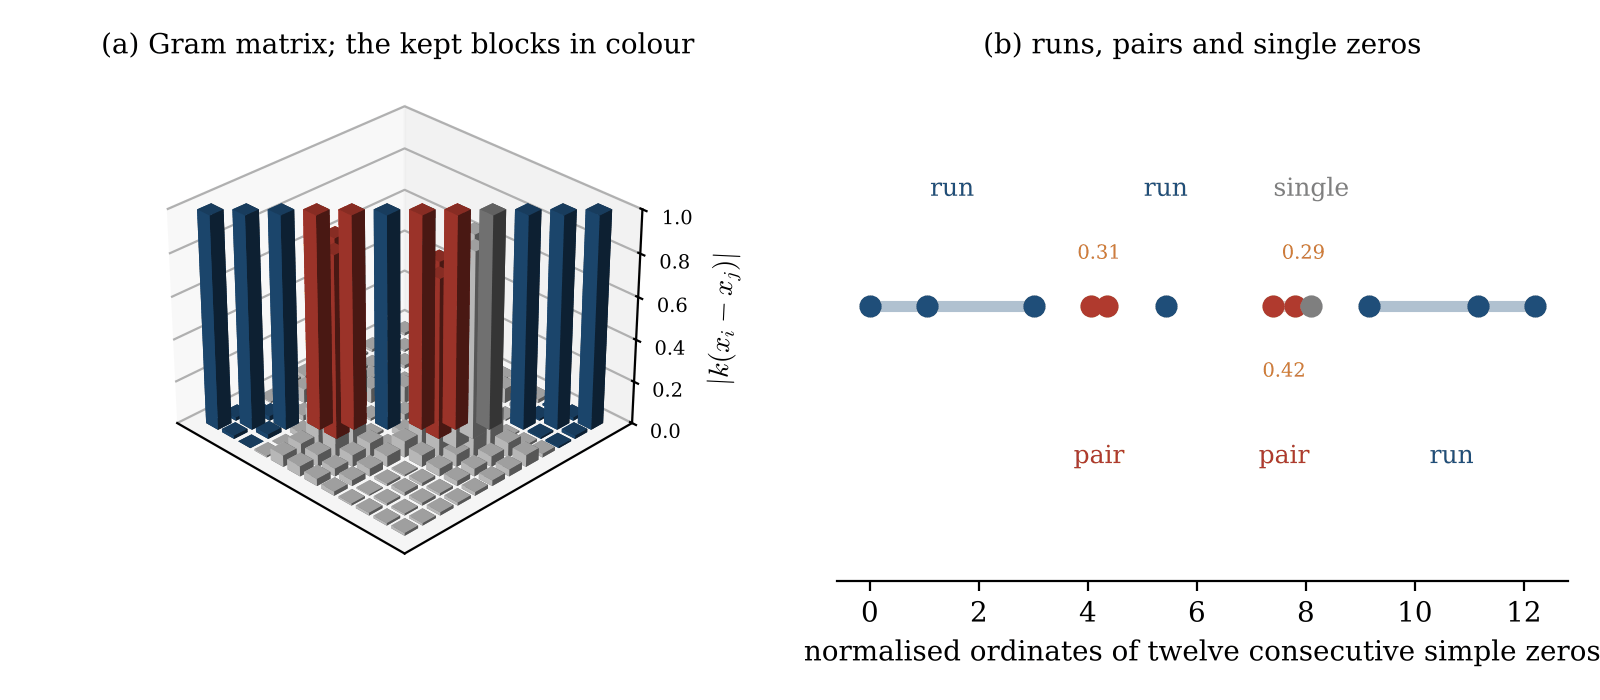
\includegraphics[width=0.96\textwidth]{figures/fig_blocks.png}
\caption{The decomposition in the proof of Proposition~\ref{prop:block},
for twelve consecutive zeros with three short gaps (orange). (a) The Gram
matrix; pinching keeps the coloured diagonal blocks and discards the grey
entries. (b) The runs have all gaps at least $\frac{11}{20}$, so their
eigenvalues stay below $2$ and their defect is their full energy; the pairs
joined by a short gap have defect at least $0.719$ each, which pays for the
windows that the clusters cut.}
\label{fig:blocks}
\end{figure*}

\section{Nine consecutive zeros}\label{sec:window}

\begin{proposition}\label{prop:window}
Let $R=9$ and let $F$ be the function~\eqref{eq:FR} with the weights of
Table~\ref{tab:weights}, whose linear total is $\mu=\frac{19999}{5000000}$. Then
\[
 F(g)\ge\frac7{1000}=0.007\qquad\text{for all }g\in[0,\infty)^8.
\]
\end{proposition}

\begin{table}[t]
\caption{The weights of Proposition~\ref{prop:window}: the pair weights
$a_{r,i}$ in units of $10^{-5}$ (row $r$, place $i$) and the linear weights
$b_{i+1}$ in units of $10^{-7}$. Both are unchanged when the window is
reversed, $a_{r,i}=a_{r,R-1-r-i}$ and $b_i=b_{R-i}$.}
\label{tab:weights}
\footnotesize\setlength{\tabcolsep}{2.3pt}
\begin{tabular}{@{}lrrrrrrrr@{}}
\toprule
 & $i=0$ & $1$ & $2$ & $3$ & $4$ & $5$ & $6$ & $7$\\
\midrule
$a_{1,i}$ & 16306 & 22126 & 28985 & 32581 & 32581 & 28985 & 22126 & 16306\\
$a_{2,i}$ & 0 & 22206 & 17667 & 120252 & 17667 & 22206 & 0 & \\
$a_{3,i}$ & 0 & 35424 & 64575 & 64575 & 35424 & 0 &  & \\
$a_{4,i}$ & 100000 & 0 & 0 & 0 & 100000 &  &  & \\
$a_{5,i}$ & 50762 & 49237 & 49237 & 50762 &  &  &  & \\
$a_{6,i}$ & 100000 & 0 & 100000 &  &  &  &  & \\
$a_{7,i}$ & 100000 & 100000 &  &  &  &  &  & \\
$a_{8,i}$ & 200000 &  &  &  &  &  &  & \\
\midrule
$b_{i+1}$ & 3188 & 4476 & 5348 & 6987 & 6987 & 5348 & 4476 & 3188\\
\bottomrule
\end{tabular}
\end{table}

\begin{figure*}[t]
\centering
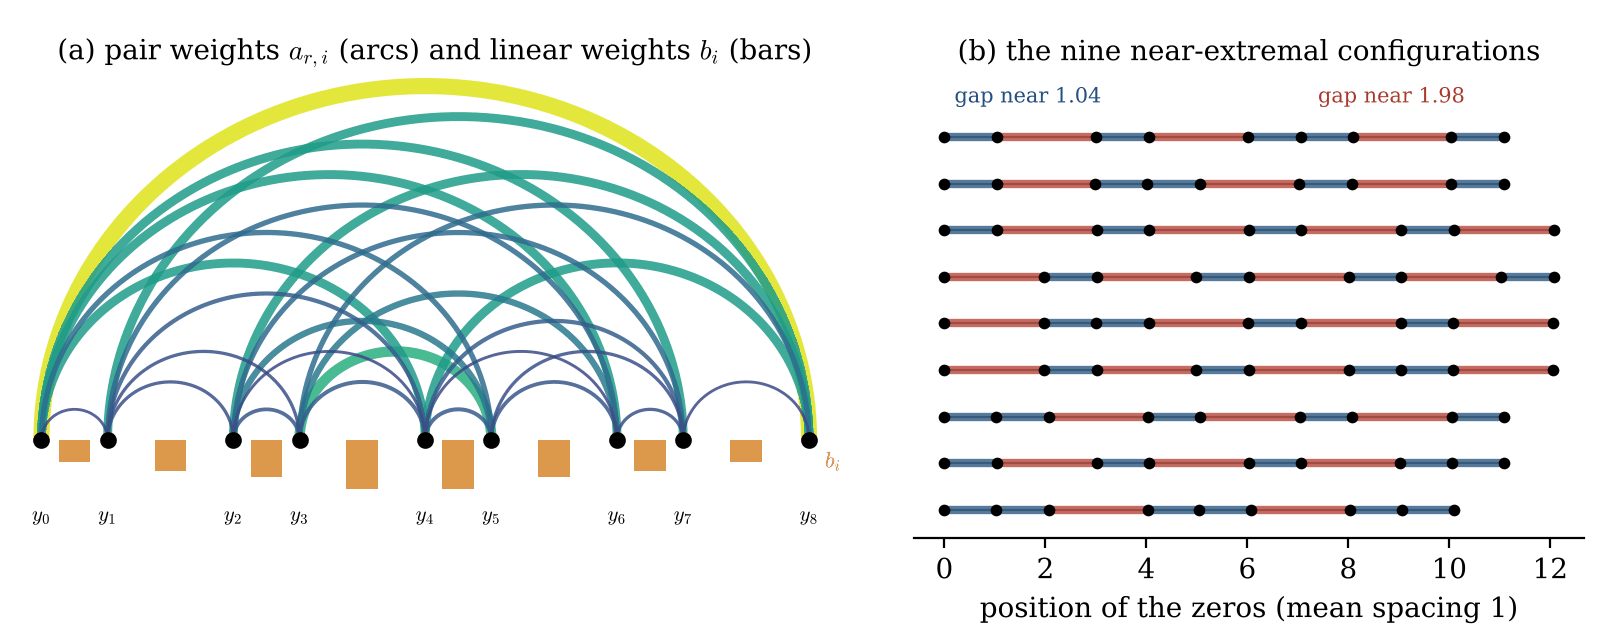
\includegraphics[width=0.96\textwidth]{figures/fig_weights.png}
\caption{(a) The weights of Table~\ref{tab:weights} over one of the
extremal configurations of Proposition~\ref{prop:window}: each arc joins
two of the nine points, with width proportional to its weight $a_{r,i}$,
and the bars below show the linear weights $b_i$. The pair at the two ends
carries the full weight $2$, and eight pairs carry none. (b) The nine gap
vectors at which $F$ comes within $3\times10^{-7}$ of its smallest value
$0.0070747$. Every gap is close to $1.04$ or to $1.97$, just above or below
a zero of $k$, and the weights are balanced so that no single arrangement
of the two gaps is cheaper than the others.}
\label{fig:weights}
\end{figure*}

The inequality is verified by a computation in rigorous arithmetic,
described in full in Appendix~\ref{app:verify}. The search covers the
whole of $[0,\infty)^8$: the linear term alone exceeds $0.007$ once
$\sum b_ig_i\ge\frac7{1000}$, and on the remaining simplex the domain is subdivided
into boxes of grid cells of width $\frac1{4000}$ until a lower bound
computed from interval enclosures of $w$ settles each box.

The weights were chosen by linear programming. For a finite set of gap
vectors, maximising the smallest value of $F$ on the set over all systems
of weights with linear total $\mu$ is a linear programme. Starting from the
uniform weights, we added the local minimisers of the current $F$ to the
set and solved the programme again, for 45 rounds, until its value and the
smallest local minimum of $F$ agreed to within $10^{-6}$; the weights were
then rounded down to the decimals of Table~\ref{tab:weights}, which keeps
\eqref{eq:weights}. The programme spreads the minimum over many
configurations: a local minimisation from many starting points finds the
smallest value $0.0070747$, attained to seven decimals at four different gap
vectors and to within $3\times10^{-7}$ at nine (Fig.~\ref{fig:weights}),
among them
\[
 (1.040,\,1.976,\,1.040,\,1.975,\,1.041,\,1.975,\,1.040,\,1.978),
\]
so the margin is $1.1$ percent. With uniform weights and the same $\mu$ the
smallest value would be $0.0068719$, which gives only $0.6731263$.\footnote{The extremal configuration is a
piece of a near-lattice: gaps of about one and two mean spacings, each
slightly larger than the zero of $k$ near $1$ or below the zero near $2$, so
that most overlaps vanish and the remaining ones balance the linear term.
Periodic arrangements of the same two gaps are the extremal chains of
Sec.~\ref{sec:limits} for values of $\mu$ near the one used here.} For
eight points the same procedure gives weights with $\mu=\frac{12499}{5000000}$
for which the verifier certifies $F\ge\frac{19}{4000}$, and hence the bound
$\frac{4000}{3981}(H_\MT-\frac{12499}{5000000})=0.6731985\ldots$. With
uniform weights the same verifier certifies $F_8\ge\frac{13}{3125}$ for
$\mu_0=\frac1{3200}$ and $F_8\ge\frac{605}{100000}$ for
$\mu_0=\frac1{2000}$, which give the weaker bounds $0.6731133\ldots$ and
$0.6730727\ldots$ by the argument of Sec.~\ref{sec:proof}.

The inequality of~\cite{Ain26} is the case $R=7$ with uniform weights,
$\mu_0=\frac1{3000}$,
$c_0=\frac{19}{5000}$. There the defect of a whole block was capped at $1$,
so blocks could contain at most about $1/c_0$ windows, and a longer window
gains nothing. Lemma~\ref{lem:eig} removes the cap, so the size of the
blocks can tend to infinity and the window length can be chosen freely.

\section{Proof of Theorem~\ref{thm:main}}\label{sec:proof}

Take $R=9$ and the weights of Proposition~\ref{prop:window}, so that
$\mu=\frac{19999}{5000000}$, and $c_0=\frac7{1000}$. Condition~\eqref{eq:c0cond} holds, since
$10c_0=0.07<0.4794<\frac43w(\frac{11}{20})$. Fix $m\ge9$ and let
$x_1<\dots<x_{S^\circ}$ be the normalised ordinates of the retained simple
zeros on the line, so that
$S^\circ=N_0^s(T,2T)-o(N(T,2T))$ by Lemma~\ref{lem:kernel}. Let $M^\circ$
be their Gram matrix.

For each offset $j\in\{0,\dots,m-1\}$, partition the points into the first
$j$ of them, consecutive blocks of $m$ points, and a final piece of fewer
than $m$ points. By Lemma~\ref{lem:pinch} and Proposition~\ref{prop:block},
\[
 \cD(M^\circ)\ge\sum_B\cD(G_B)
 \ge\sum_B\bigl(c_0(m-R+1)-\mu\spanop(B)-o(1)\bigr).
\]
For every offset there are at least $S^\circ/m-2$ blocks and at most
$S^\circ/m$, and the $o(1)$ is uniform, so these terms total $o(N)$, with
$N=N(T,2T)$. Average over the $m$ offsets. A gap $x_{i+1}-x_i$ lies inside a
block for at most $m-1$ of the $m$ offsets, and
$x_{S^\circ}-x_1\le d=N\,(1+O(1/L))$, so
\[
 \cD(M^\circ)\ge\frac{c_0(m-R+1)}m\,S^\circ-\frac{(m-1)\mu}m\,N-o(N).
\]
Insert this in Corollary~\ref{cor:defect}:
\begin{align*}
 &\Bigl(1-\frac{c_0(m-R+1)}m\Bigr)N_0^s(T,2T)\\
 &\qquad\ge\Bigl(H_\MT-\frac{(m-1)\mu}m\Bigr)N-o(N).
\end{align*}
Divide by $N$ and let $T\to\infty$, and then let $m\to\infty$:
\[
 \liminf_{T\to\infty}\frac{N_0^s(T,2T)}{N(T,2T)}\ge
 \frac{H_\MT-\mu}{1-c_0}=\frac{1000}{993}\Bigl(H_\MT-\frac{19999}{5000000}\Bigr).
\]
The value is $0.6732133974616431\ldots$, computed in ball
arithmetic~\cite{Joh17}. \hfill$\square$

\begin{remark}
Every input of the proof is available for a Dirichlet $L$-function
$L(s,\chi)$ with $\chi$ primitive: Proposition~\ref{prop:AF} holds there
by~\cite[Theorem~B]{AF26}, and Lemmas~\ref{lem:stable}--\ref{lem:windows}
do not involve $\zeta$. The same constant therefore holds for the simple
zeros of $L(s,\chi)$ on the critical line.
\end{remark}

\section{How far the method goes}\label{sec:limits}

The argument has three parameters: the window length $R$, the weights,
with linear total $\mu$, and the constant $c_0$, which is the minimum of
$F$. Longer windows and better weights see more of the energy. With
uniform weights the local minima of $F_R$ give about $0.67309$, $0.67313$
and $0.67317$ for $R=7$, $8$ and $9$, while optimised weights reach
$0.67321$ with $R=8$ and $0.67326$ with $R=9$. The following
proposition bounds what any window and any weights can give.

\begin{proposition}\label{prop:limit}
Let $(g_i)_{i\in\Z}$ be a periodic sequence of positive gaps with period
$p$ and mean $\bar g$, let $y$ be the corresponding points, and put
\[
 e(g,\mu)=\mu\bar g+\frac2p\sum_{i=1}^p\sum_{j>i}w(y_j-y_i).
\]
If $F\ge c_0$ holds for a system of weights with linear total $\mu$, then
$c_0\le e(g,\mu)$, and
the bound obtained in Sec.~\ref{sec:proof} is at most
$(H_\MT-\mu)/(1-e(g,\mu))$.
\end{proposition}

\begin{proof}
Apply Lemma~\ref{lem:windows} to $n$ consecutive points of the sequence,
divide by $n$ and let $n\to\infty$; the double sum converges because
$w(x)=O(x^{-2})$.
\end{proof}

Minimising $e(g,\mu)$ over periodic patterns of period at most $4$ on a
grid of weights gives the values in Table~\ref{tab:chain}. For a fixed
pattern the upper limit $(H_\MT-\mu)/(1-e(g,\mu))$ is monotone in $\mu$,
since its derivative has the sign of $\bar gH_\MT+e(g,0)-1$, so the
patterns found at the grid points bound it on every interval between
them.\footnote{The double sum is taken over all pairs: $2\times10^5$
neighbours are summed and the rest is bounded by
$|k(x)|\le(K_0(\pi x-1/\sqrt2))^{-1}$. A truncation at a few hundred
neighbours, which looks harmless because $w$ is small there, lowers
$e(g,\mu)$ by about $5\times10^{-5}$, more than the margins in the table.}
The resulting bound stays below $0.67357$ for every $\mu\ge0$, with the
largest value near $\mu=0.0061$, where the best pattern is the alternation
$(1.036,1.964)$; for smaller $\mu$ gaps near $2$ take over, and for larger
$\mu$ patterns with more gaps near $1$. So no window length or choice of
weights improves Theorem~\ref{thm:main} by more than $0.0004$, and the
approach cannot reach $67.36$ percent. The proof of
Proposition~\ref{prop:limit} uses only the pairs at most $R-1$ steps apart,
so the double sum may be restricted to them; for $R=9$ and $\mu=0.004$
the restricted chain energy gives the limit $0.6732646$ for nine points,
and the weights of Table~\ref{tab:weights} come within $10^{-6}$ of it
before rounding. Longer windows gain slowly: at the same $\mu$ the limit is
$0.6732908$ for ten points and $0.6733252$ for twelve. Tilting
the window, that is replacing $\cos(\sqrt2t)$ by $\cos(\alpha t)$, lowers
$H_\MT$ faster than it raises the defect: at $R=7$ the best tilt,
$\alpha=1.5$, gains $0.00004$.

\begin{table}[t]
\caption{The chain energy $e(\mu)$, the smallest value of $e(g,\mu)$ found
over periodic gap patterns $g$ of period at most $4$, the pattern that
attains it, and the resulting upper limit $(H_\MT-\mu)/(1-e(\mu))$ for the
bound of Sec.~\ref{sec:proof}.}
\label{tab:chain}
\begin{tabular}{@{}lccc@{}}
\toprule
$\mu$ & $e(\mu)$ & pattern & upper limit\\
\midrule
$0.0020$ & $0.0043102$ & $(1.99,1.98,1.04,1.98)$ & $0.6734032$\\
$0.0025$ & $0.0051570$ & $(1.98,1.04,1.98)$ & $0.6734738$\\
$0.0030$ & $0.0059725$ & $(1.04,1.96)$ & $0.6735233$\\
$0.0040$ & $0.0074727$ & $(1.04,1.96)$ & $0.6735338$\\
$0.0050$ & $0.0089729$ & $(1.04,1.96)$ & $0.6735443$\\
$0.0060$ & $0.0104731$ & $(1.04,1.96)$ & $0.6735549$\\
$0.0065$ & $0.0111605$ & $(1.02,1.02,1.95)$ & $0.6735175$\\
$0.0080$ & $0.0131609$ & $(1.02,1.02,1.95)$ & $0.6733628$\\
\bottomrule
\end{tabular}
\end{table}

Going further needs information that the energy of runs does not see.
Alp\"oge and Furman show that no certificate built from pair correlation
with Fourier support in $[-1,1]$ can exceed about
$0.6818$~\cite[\S7.2]{AF26}. Between $0.6736$ and $0.6818$ lies the part of
that information which the stability defect, a function of the Gram matrix
of the simple zeros alone, does not capture. Information beyond pair
correlation can raise the ceiling: in the periodic models of~\cite[\S7.2]{AF26}
with the three-point correlations of the circular unitary ensemble added,
the ceiling rises to about $0.709$. These correlations are known in the
range used, but an off-line pair of zeros enters a triple product with a
weight that grows faster than in the quadratic case, and the known
zero-density estimates control only the triples whose frequencies add up to
less than half of the range. With those alone the gain is about $0.0002$.

None of this bears on the Riemann hypothesis itself. Every bound of this
kind is insensitive to a set of zeros of density zero, and the
argument applies equally to functions, such as the Davenport--Heilbronn
function, whose zeros are known to leave the critical line.

\section*{Data and code availability}

The proofs of Lemmas~\ref{lem:stable}--\ref{lem:windows} and of
Proposition~\ref{prop:block} are by hand. Proposition~\ref{prop:window} is
verified by the rigorous computation described in Appendix~\ref{app:verify}.
The repository \texttt{creelie/mh-phys} contains the \LaTeX{} source of this
paper; the table of interval enclosures of $w$ in 128-bit ball arithmetic
with its hash; the branch-and-bound verifier, in serial, parallel and weighted
versions, with the weights of Table~\ref{tab:weights} and the logs of the certified runs and a workflow that repeats the
certificate on every change; independent checks in ball and floating-point
arithmetic of the eigenvalue bound, of the endpoint values in
Appendix~\ref{app:details} and of the eigenvalues of lattices; the local
minimisations for $R=7,8,9$ and the linear programmes that choose the
weights; the chain energies of Table~\ref{tab:chain} and
their extension to every weight; the linear programmes behind the ceilings
quoted in Sec.~\ref{sec:limits}; and the failure log of the search that led
to the argument. The archive
is~\cite{Archive}, \archivelink, where later versions are listed. The search followed the learn-from-failure protocol of
the BLLM engine Anaxia, release~3.0.5~\cite{Ana26}. Deep Bhattacharjee
carried out the computations and the C, Python and shell checks with AI
assistance from Claude (Anthropic); both authors approved the final text.

\section*{Ethical declarations}

\emph{Funding.} None. \emph{Competing interests.} None.

\appendix

\section{Elementary estimates}\label{app:details}

\subsection{The majorant}

We prove~\eqref{eq:majorant}. Both sides are even, so let
$0\le t\le\frac12$ and $s=\pi\delta_1t\in[0,0.8640]$. The Taylor series
\[
 \sinc^2s=\frac{1-\cos2s}{2s^2}=\sum_{k\ge1}(-1)^{k+1}
 \frac{2^{2k-1}s^{2k-2}}{(2k)!}
\]
alternates, and for $s\le1$ the ratio of consecutive terms is
$4s^2/((2k+1)(2k+2))<1$, so the terms decrease in absolute value and the
partial sum ending with a negative term is a lower bound:
\[
 \sinc^2s\ge1-\frac{s^2}3+\frac{2s^4}{45}-\frac{s^6}{315}.
\]
In the same way $\cos y\le1-\frac{y^2}2+\frac{y^4}{24}$ for all real $y$.
With $y=\sqrt2\,t$ and $u=t^2\in[0,\frac14]$,
\begin{gather*}
 \Lambda(t)-\cos(\sqrt2\,t)\ge-u\,q(u),\\
 q(u)=(\alpha_1-1)+\bigl(\tfrac16-\alpha_2\bigr)u+\alpha_3u^2,
\end{gather*}
where $\alpha_1=(\pi\delta_1)^2/3=0.9951851\ldots$,
$\alpha_2=2(\pi\delta_1)^4/45=0.3961573\ldots$ and
$\alpha_3=(\pi\delta_1)^6/315=0.0844821\ldots$. The quadratic $q$ is convex,
so its maximum on $[0,\frac14]$ is at an endpoint, and
\[
 q(0)=-0.0048148\ldots<0,\qquad q(\tfrac14)=-0.0569074\ldots<0.
\]
Hence $\Lambda(t)\ge\cos(\sqrt2t)$ on $[0,\frac12]$. The values are computed
with $\pi$ enclosed in 200-bit ball arithmetic; $q(0)=\alpha_1-1$ alone
needs only $\pi^2\cdot0.3025<3$, that is $\pi^2<9.918$. The margin at small
$t$ is of order $0.0048\,t^2$, which is why $\delta_1$ cannot be lowered
much: $q(0)<0$ requires $\delta_1<\sqrt3/\pi=0.5513$.

\subsection{The Fourier transform of the Fej\'er kernel}

For $\Delta>0$, the triangle $\tau(\xi)=\Delta^{-1}(1-|\xi|/\Delta)_+$ is
the convolution of $\Delta^{-1}\mathbf 1_{[-\Delta/2,\Delta/2]}$ with itself,
whose inverse Fourier transform is $\sinc(\pi\Delta t)$. Hence
$\int\tau(\xi)e^{-2\pi i\xi t}\,d\xi=\sinc^2(\pi\Delta t)$, and Fourier
inversion gives the formula used in the proof of Lemma~\ref{lem:eig}.

\subsection{Values of the kernel}

From~\eqref{eq:Kexplicit}, in 200-bit ball arithmetic,
\begin{align*}
 K_0&=0.91872536986556843778\ldots,\\
 1/(\delta_1K_0)&=1.97902646189890434914\ldots,\\
 k(\tfrac{11}{20})&=0.59963660635252251069\ldots,\\
 w(\tfrac{11}{20})&=0.35956405967797003982\ldots,
\end{align*}
so that $\frac43w(\frac{11}{20})=0.4794187\ldots$. The minimum of $k$ on
$[0,\infty)$ is $-0.1804\ldots$, attained near $x=1.47$.

\subsection{Convex trace functions}

If $f$ is convex on an interval $J$, then $X\mapsto\tr f(X)$ is convex on
the Hermitian matrices with spectrum in $J$~\cite[Theorem V.2.5]{Bha97}.
For the pinching we need it on positive semidefinite matrices, with
$f=\Psi$; the averages $2^{-q}\sum_\varepsilon U_\varepsilon XU_\varepsilon$
of Lemma~\ref{lem:pinch} remain positive semidefinite, so the spectrum stays
in $[0,\infty)$, where $\Psi$ is convex.

\section{Verification of Proposition~\ref{prop:window}}\label{app:verify}

\subsection{The table}

For $c=0,1,\dots,79999$, a lower bound $\underline w_c$ for $w$ on the cell
$[c/4000,(c+1)/4000]$ is computed by evaluating~\eqref{eq:Kexplicit} on the
cell as a ball in 128-bit arithmetic~\cite{Joh17}, taking the lower bound of
$|k|$, rounding it down to a double, squaring, and rounding down again. On
$[20,\infty)$ only $w\ge0$ is used. The table occupies $640{,}000$ bytes
and has SHA-256 hash \texttt{fd9304e3\ldots}; its first $46{,}000$ cells
form the table of hash \texttt{8ea9e020\ldots}, used for the uniform
weights. Both hashes are recorded in full in the archive.

\subsection{Rounding}

All floating-point operations of the verifier run in the rounding mode
towards $-\infty$, on nonnegative quantities, so that every computed sum and
product is a lower bound for the exact one. The target $\frac7{1000}$ is
rounded up; every weight, stored as a quotient of integers, is rounded
down, and so is $b_i/4000$.

\subsection{Reduction to a compact region}

If the lower ends $l_i$ of the cells that contain the gaps satisfy
$\sum_i(b_i/4000)\,l_i\ge\frac7{1000}$, the linear term alone settles the
inequality. In particular the gap $g_i$ is confined to the cells below
$C_i$, the least integer with $(b_i/4000)\,C_i\ge\frac7{1000}$; here
$C_1=C_8=87{,}830$, $C_2=C_7=62{,}556$, $C_3=C_6=52{,}357$ and
$C_4=C_5=40{,}075$. Moreover every single gap satisfies
$b_ig_i+a_{1,i-1}w(g_i)<\frac7{1000}$, since all other terms are
nonnegative. Testing this cell by cell leaves one or two intervals of cells
for each gap: $[3451,87829]$ for $g_1$ and $g_8$; $[3555,5472]$ and
$[6347,61984]$ for $g_2$ and $g_7$; $[3635,5164]$ and $[6713,52310]$ for
$g_3$ and $g_6$; and $[3671,5059]$ and $[6853,40072]$ for $g_4$ and $g_5$.
The $64$ products of these intervals are the initial boxes.

\subsection{Lower bound on a box}

A box is a product of intervals of cells $[l_i,u_i]$, $i=1,\dots,8$. On it,
$\sum b_ig_i\ge\sum(b_i/4000)\,l_i$, and the distance $y_{i+r}-y_i$ lies
in the union of the cells from $\sum l$ to $\sum(u+1)-1$ over the $r$ gaps
involved. The minimum of $\underline w_c$ over that range of cells, found by
a sparse table of range minima, bounds $w$ from below. Adding these bounds
with their weights gives a lower bound for $F$ on the box. A box is
discarded when this bound reaches $\frac7{1000}$; otherwise its widest
coordinate interval is halved. The verification fails if a box consisting
of single cells is not discarded.

\subsection{The run}

The boxes are first split breadth-first until $2{,}331{,}717$ remain, and
these are then processed depth-first, in parallel, with the rounding mode
set in each thread; a thread that runs out of boxes takes half of the stack
of a busy one. The search examined $52{,}891{,}178{,}741$ boxes in about 30
minutes on four threads of a four-core processor and discarded all of them.
For eight points, the weights with $\mu=\frac{12499}{5000000}$ give
$F\ge\frac{19}{4000}$ after $21{,}067{,}790{,}614$ boxes. With uniform
weights the same program
certifies $F_8\ge\frac{13}{3125}$ for $\mu_0=\frac1{3200}$ after
$10{,}039{,}560{,}518$ boxes, using the table of $46{,}000$ cells. The run for
$\mu_0=\frac1{2000}$ and $c_0=\frac{605}{100000}$, made with the serial
version, examined $5{,}440{,}924{,}378$ boxes. The same verifier reproduces
the inequality of~\cite{Ain26} for $R=7$, $\mu_0=\frac1{3000}$,
$c_0=\frac{19}{5000}$, with the same three intervals of cells.

\begin{thebibliography}{99}\raggedright\advance\leftskip\labelwidth

\bibitem{Ain26}
ainta, A $67.30085\%$ lower bound for simple zeros of the Riemann zeta
function, GitHub repository \nolinkurl{ainta/zeta-simple-zeros} (2026),
mirrored at \url{https://github.com/creelie/zeta-simple-zeros}.

\bibitem{AF26}
L.~Alp\"oge and R.~Furman, More than two thirds of the zeta zeros are simple
and on the critical line, preprint (2026),
\href{https://arxiv.org/abs/2608.13637}{arXiv:2608.13637}.

\bibitem{BGSTB24}
S.~A.~C. Baluyot, D.~A. Goldston, A.~I. Suriajaya and C.~L.
Turnage-Butterbaugh, An unconditional Montgomery theorem for pair
correlation of zeros of the Riemann zeta-function, Acta Arith. \textbf{214}
(2024), 357--376,
\href{https://doi.org/10.4064/aa230612-20-3}{doi:10.4064/aa230612-20-3}.

\bibitem{Bha97}
R.~Bhatia, \emph{Matrix Analysis}, Grad. Texts in Math. 169, Springer, New
York, 1997,
\href{https://doi.org/10.1007/978-1-4612-0653-8}{doi:10.1007/978-1-4612-0653-8}.

\bibitem{BB26a}
D.~Bhattacharjee and U.~Bhattacharya, Maximal large sieve and coefficient
uniform failure for Liouville correlations, Preprints (2026),
\href{https://doi.org/10.20944/preprints202606.1350.v1}{doi:10.20944/preprints202606.1350.v1}.

\bibitem{BB26c}
D.~Bhattacharjee and U.~Bhattacharya, BLLM: Beyond the LLM with Deep
Human-Mind-AI, preprint (2026), distributed with~\cite{Ana26}.

\bibitem{BNFS26}
D.~Bhattacharjee, P.~Nandi, O.~Frederick and P.~Samal, Spectral and
analytic structure of the Nyman--Beurling--B\'aez-Duarte approximation,
Preprints (2026),
\href{https://doi.org/10.20944/preprints202506.0772.v2}{doi:10.20944/preprints202506.0772.v2}.

\bibitem{Ana26}
D.~Bhattacharjee, Anaxia, the BLLM engine, eBLLM release 3.0.5, Zenodo
(2026), \href{https://doi.org/10.5281/zenodo.23469389}{doi:10.5281/zenodo.23469389};
all versions
\href{https://doi.org/10.5281/zenodo.23286641}{doi:10.5281/zenodo.23286641}.

\bibitem{BCY11}
H.~M. Bui, J.~B. Conrey and M.~P. Young, More than $41\%$ of the zeros of
the zeta function are on the critical line, Acta Arith. \textbf{150}
(2011), 35--64,
\href{https://doi.org/10.4064/aa150-1-3}{doi:10.4064/aa150-1-3}.

\bibitem{CCLM17}
E.~Carneiro, V.~Chandee, F.~Littmann and M.~B. Milinovich, Hilbert spaces
and the pair correlation of zeros of the Riemann zeta-function, J. Reine
Angew. Math. \textbf{725} (2017), 143--182,
\href{https://doi.org/10.1515/crelle-2014-0078}{doi:10.1515/crelle-2014-0078}.

\bibitem{Con89}
J.~B. Conrey, More than two fifths of the zeros of the Riemann zeta function
are on the critical line, J. Reine Angew. Math. \textbf{399} (1989), 1--26,
\href{https://doi.org/10.1515/crll.1989.399.1}{doi:10.1515/crll.1989.399.1}.

\bibitem{HB79}
D.~R. Heath-Brown, Simple zeros of the Riemann zeta-function on the
critical line, Bull. London Math. Soc. \textbf{11} (1979), 17--18,
\href{https://doi.org/10.1112/blms/11.1.17}{doi:10.1112/blms/11.1.17}.

\bibitem{Joh17}
F.~Johansson, Arb: efficient arbitrary-precision midpoint-radius interval
arithmetic, IEEE Trans. Comput. \textbf{66} (2017), 1281--1292,
\href{https://doi.org/10.1109/TC.2017.2690633}{doi:10.1109/TC.2017.2690633}.

\bibitem{Lam26}
Y.~Lamzouri, A new proof that more than $2/3$ of the zeros of the Riemann
zeta function are simple and on the critical line, preprint (2026),
\href{https://arxiv.org/abs/2609.02882}{arXiv:2609.02882}.

\bibitem{Lev74}
N.~Levinson, More than one third of zeros of Riemann's zeta-function are on
$\sigma=\frac12$, Adv. Math. \textbf{13} (1974), 383--436,
\href{https://doi.org/10.1016/0001-8708(74)90074-7}{doi:10.1016/0001-8708(74)90074-7}.

\bibitem{Mon73}
H.~L. Montgomery, The pair correlation of zeros of the zeta function, in
\emph{Analytic Number Theory}, Proc. Sympos. Pure Math. 24, Amer. Math.
Soc., Providence, 1973, 181--193,
\href{https://doi.org/10.1090/pspum/024/9944}{doi:10.1090/pspum/024/9944}.

\bibitem{Mon75}
H.~L. Montgomery, Distribution of the zeros of the Riemann zeta function,
in \emph{Proceedings of the International Congress of Mathematicians
(Vancouver, 1974)}, Vol.~1, Canad. Math. Congress, Montreal, 1975, 379--381.

\bibitem{PRZZ20}
K.~Pratt, N.~Robles, A.~Zaharescu and D.~Zeindler, More than five-twelfths
of the zeros of $\zeta$ are on the critical line, Res. Math. Sci.
\textbf{7} (2020), Paper No.~2,
\href{https://doi.org/10.1007/s40687-019-0199-8}{doi:10.1007/s40687-019-0199-8}.

\bibitem{Sel42}
A.~Selberg, On the zeros of Riemann's zeta-function, Skr. Norske
Vid.-Akad. Oslo I \textbf{1942}, no.~10, 1--59.

\bibitem{Tit86}
E.~C. Titchmarsh, \emph{The Theory of the Riemann Zeta-Function}, 2nd ed.,
revised by D.~R. Heath-Brown, Clarendon Press, Oxford, 1986.

\bibitem{Vaa85}
J.~D. Vaaler, Some extremal functions in Fourier analysis, Bull. Amer.
Math. Soc. (N.S.) \textbf{12} (1985), 183--216,
\href{https://doi.org/10.1090/S0273-0979-1985-15349-2}{doi:10.1090/S0273-0979-1985-15349-2}.

\bibitem{Wei52}
A.~Weil, Sur les ``formules explicites'' de la th\'eorie des nombres
premiers, Comm. S\'em. Math. Univ. Lund, tome suppl\'ementaire (1952),
252--265.

\bibitem{Archive}
D.~Bhattacharjee and U.~Bhattacharya, Simple zeros on the critical line:
source, verifier and certificates, \ifx\zenodoID\empty GitHub repository
\texttt{creelie/mh-phys}\else Zenodo\fi{} (2026), \archivelink.

\end{thebibliography}

\end{document}
